\chapter{Negative Sampling模型}

在负采样中,对于给定的词$w$,如何生成它的负采样集合$NEG(w)$呢?
已知一个词$w$,它的上下文是$context(w)$,那么词$w$就是一个正例,
其他词就是一个负例。但是负例样本太多了,我们怎么去选取呢?
在语料库$\mathcal{C}$中,各个词出现的频率是不一样的,
我们采样的时候要求高频词选中的概率较大,而低频词选中的概率较小。
这就是一个带权采样的问题。
设词典$\mathcal{D}$中的每一个词$w$对应线段的一个长度:
\begin{equation}
    len(w) = \frac{counter(w)}{\sum_{u \in \mathcal{D}}counter(u)} (1)
\end{equation}
式4.1分母是为了归一化,Word2Vec中的具体做法是:
记$l_0 = 0, l_k = \sum_{j=1}^{k} len(w_j), k=1,2, \dots, N$,
其中,$w_j$是词典$\mathcal{D}$中的第$j$个词,
则以$\{l_j\}_{j=0}^{N}$为点构成了一个在区间[0,1]非等距离的划分。
然后再加一个等距离划分,Word2Vec中选取$M=10^8$,将M个点等距离的分布在区间[0,1]上,
这样就构成了M到I之间的一个映射,如下图所示:
\begin{figure}[h]
    \begin{center}
        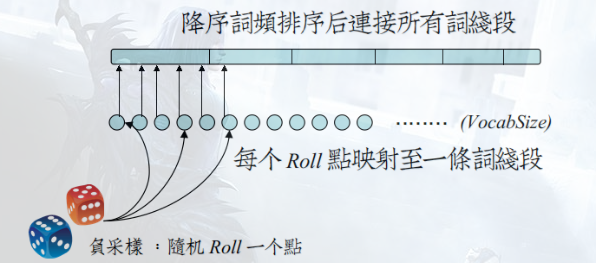
\includegraphics[width=12cm, height=6cm]{4_1}
        \caption{负采样}
    \end{center}
\end{figure}

图例参考:
\href{http://www.cnblogs.com/neopenx/p/4571996.html}{\textbf{建议大家读下这篇神作}}。

选取负例样本的时候,取$[M_0, M_{m-1}]$上的一个随机数,对应到I上就可以了。
如果对于词$w_i$,正好选到它自己,则跳过。负例样本集合$NEG(w)$的大小在Word2Vec源码中默认选5.

\section{CBOW}
假定关于词$w$的负例样本$NEG(w)$已经选出,定义标签$L$如下,
对于 $\forall \widetilde{w} \in \mathcal{D}$:
\begin{equation}
    L^w(\widetilde{w}) = \Bigg\{ \begin{array} {ll}
        1,  & \widetilde{w} = w ;\\
        0, & \widetilde{w} \ne w;
        \end{array}
\end{equation}

对于给定的一个正例样本$(context(w), w)$, 要求:
\begin{equation}
    \max g(w) = \max \prod_{u \in \{w\} \cup u \in NEG(w)} p(u|context(w))
\end{equation}

其中, 
\begin{equation}
    p(u|context(w)) = \Bigg \{ \begin{array}{ll}
        \sigma(\boldsymbol{x}_w^T \theta^u), & L^w(u) = 1\\
        1-\sigma(\boldsymbol{x}_w^T \theta^u), & L^w(u) = 0
        \end{array}
\end{equation}

把它写成一个式子:
\begin{equation}
    p(u|context(w)) = \sigma(\boldsymbol{x}_w^T \theta^u)^{L^w(u)} + (1-\sigma(\boldsymbol{x}_w^T \theta^u))^{1-L^w(u)}
\end{equation}

下边解释为什么要最大化$g(w)$,
\begin{equation}
    \begin{split}
        g(w) &= \prod_{u \in \{w\} \cup u \in NEG(w)} p(u|context(w)) \\
        &=\prod_{u \in \{w\} \cup u \in NEG(w)}  \sigma(\boldsymbol{x}_w^T \theta^u)^{L^w(u)} + (1-\sigma(\boldsymbol{x}_w^T \theta^u))^{1-L^w(u)} \\ 
        &=\sigma(\boldsymbol{x}_w^T \theta^w)\prod_{u \in NEG(w)} (1-\sigma(\boldsymbol{x}_w^T \theta^u))
    \end{split}
\end{equation}

\textbf{上式中连乘号前边的式子可以解释为最大化正例样本概率,连乘号后边解释为最小化负例样本概率}。

同样的,针对于语料库,令:
\begin{equation}
    \mathcal{G} = \prod_{w \in \mathcal{C}} g(w)
\end{equation}

可以将上式作为整体的优化目标函数,取上式的最大似然:
\begin{equation}
    \begin{split}
    \mathcal{L} = \log\mathcal{G} \\
    &= \sum_{w \in \mathcal{C}} \log g(w) \\
    &=\sum_{w \in \mathcal{C}} \sum_{u \in \{w\} \cup u \in NEG(w)}L^w(u)\log[\sigma(\boldsymbol{x}_w^T \boldsymbol{\theta}^u] + [1-L^w(u)]
    \log [1-\sigma(\boldsymbol{x}_w^T \boldsymbol{\theta}^u)]
\end{split}
\end{equation}

和之前的计算过程一样,记
\begin{equation}
    L(w,u) = L^w(u)\log[\sigma(\boldsymbol{x}_w^T \theta^u] + [1-L^w(u)]\log [1-\sigma(\boldsymbol{x}_w^T \boldsymbol{\theta}^u)]
\end{equation}

然后分别求:$\frac{\partial L(w,u)}{\partial\boldsymbol{X}_w}$和$\frac{\partial L(w,u)}{\partial\boldsymbol{\theta}^u}$,求解过程略过:
\begin{equation}
    \frac{\partial L(w,u)}{\partial\boldsymbol{X}_w} = [L^w(u)-\sigma(\boldsymbol{x}_w^T \boldsymbol{\theta}^u)]\boldsymbol{\theta}^u 
\end{equation}
\begin{equation}
    \frac{\partial L(w,u)}{\partial\boldsymbol{\theta}^u} = [L^w(u)-\sigma(\boldsymbol{x}_w^T \boldsymbol{\theta}^u)]\boldsymbol{X}_w
\end{equation}
则,可得到如下更新公式:
\begin{equation}
    \boldsymbol{\theta}^u:=\boldsymbol{\theta}^u+\eta [L^w(u)-\sigma(\boldsymbol{x}_w^T \boldsymbol{\theta}^u)]\boldsymbol{X}_w \\
\end{equation}
\begin{equation}
    v(\boldsymbol{\widetilde{w}}):=v(\boldsymbol{\widetilde{w}}) + \sum_{u \in \{w\} \cup u \in NEG(w)} [L^w(u)-\sigma(\boldsymbol{x}_w^T \boldsymbol{\theta}^u)]\boldsymbol{\theta}^u
\end{equation}
其中, $\boldsymbol{\widetilde{w}} \in context(w)$.

\section{Skip-gram模型}
这部分内容并不多,与cbow相比,只是目标函数有所变化,推导过程这里就略过。
总的来说,就是将目标函数取最大似然,然后利用SGD方法求出词向量和最优参数。
目标函数如下所示:
\begin{equation}
    G = \prod_{w \in \mathcal{C}} g(w)
\end{equation}
其中,$g(w)$可以改写成如下形式:
\begin{equation}
    g(w)=\prod_{u \in context(w)} g(u)
\end{equation}
$g(u)$表示如下:
\begin{equation}
    g(u) = \prod_{z \in \{u\} \cup NEG(u)} p(z|w)
\end{equation}
其中,$NEG(u)$表示在处理词$u$时产生的负样本集合。$p(z|w)$如下:
\begin{equation}
    p(z|w) = \Bigg \{ \begin{array}{ll}
    \sigma(\boldsymbol{v(w)}^T \theta^z), & L^u(z) = 1\\
    1-\sigma(\boldsymbol{v(w)}^T \theta^z), & L^u(z) = 0
    \end{array}
\end{equation}
将以上式子合并之后就可以得到最终的目标函数:
\begin{equation}
    G = \prod_{w \in \mathcal{C}}\prod_{u \in context(w)}\prod_{z \in \{u\} \cup NEG(u)} \sigma(\boldsymbol{v(w)}^T \theta^z)^{L^u(z)}(1-\sigma(\boldsymbol{v(w)}^T \theta^z))^{L^u(z)}
\end{equation}
然后取$G$的最大似然对数,求目标函数的最优化。

 